\chapter{El microprocesador}\label{chapter:microprocesador}

El \textbf{microprocesador} es un \textbf{procesador} de computadora, donde la lógica del procesamiento de datos y el control
están incluidos en un solo circuito integrado, o en un pequeño número de circuitos integrados. El circuito integrado es capaz 
de interpretar y ejecutar instrucciones de programa y realizar operaciones aritméticas. El \textbf{microprocesador} es un 
circuito integrado digital multipropósito, controlado por reloj y basado en registros que acepta datos binarios como entrada, 
los procesa de acuerdo con las instrucciones almacenadas en su memoria y proporciona resultados (también en forma binaria) 
como salida. Un \textbf{microprocesador} hipotético mínimamente funcional podría incluir solo una \textbf{ALU}(\emph{Arithmetic Logic Unit}) 
y una sección lógica de control. La \textbf{ALU} realiza sumas, restas y operaciones como \textbf{AND} y \textbf{OR}. Cada operación de la
\textbf{ALU} establece uno o más \emph{flags} en un registro de estados, que indican los resultados de la última operación
(por ejemplo, si el resultado es cero, si es negativo, si hay desbordamiento, etc.). La lógica de control recupera los
código de instrucción desde la memoria e inicia la secuencia de operaciones necesarias para que la \textbf{ALU} lleve a
cabo la instrucción \brackcite{wikipedia_2022_Microprocesador}.\\ Antes de los microprocesadores las computadoras pequeñas
se construían utilizando  \emph{racks} de placas de circuito con muchos circuitos integrados de mediana y pequeña escala,
generalmente del tipo \textbf{TTL}\emph{(Transistor-Transistor Logic)} \brackcite{wikipedia_2022_ttl}. Los microprocesadores
combinaron esto en uno o unos pocos circuitos integrados a gran escala.\\ El incremento continuo de las capacidades de los
microprocesadores desde  que se empezaron a fabricar ha dejado otras formas de computadoras casi complemtamente obsoletas,
con uno o más microprocesadores usados en todo desde pequeños sistemas embebidos y dispostivos portátiles hasta en los enormes
\emph{mainframes} y supercomputadoras.

\section{Surgimiento del microprocesadaor}
Las invenciones a veces ocurren cuando las personas se enfrentan a un problema y luchan por resolverlo. En otras ocasiones, suceden 
cuando las personas adoptan una meta visionaria. La historia de cómo \emph{Ted Hoff} y su equipo de \emph{Intel} inventaron el \textbf
{microprocesador} es un caso de ambos \brackcite{isaacson_2014}. \emph{Hoff}, que había sido un joven profesor en \emph{Stanford}, se
convirtió en el duodécimo empleado de \emph{Intel}, donde fue asignado para trabajar en el diseño de chips. \emph{Hoff} se dió cuenta de que era un
desperdicio y poco elegante diseñar muchos tipos de \emph{microchips} donde cada uno tuviera una función diferente,  que era lo que \emph{Intel} 
estaba haciendo hasta ahora. Llegaría una empresa y le pediría que construyera un \emph{microchip} diseñado para realizar una tarea
específica. \emph{Hoff} imaginó, al igual que \emph{Noyce} y otros, un enfoque alternativo: crear un \emph{chip} de propósito general que pudiera
ser instruido o programado para realizar una variedad de aplicaciones diferentes según se desee. En otras palabras, una computadora de propósito
general en un \emph{chip}. Esta visión coincidió con un problema que se planteó a \emph{Hoff} en el verano de 1969. Una empresa japonesa llamada
\emph {Busicom} estaba planeando una nueva y poderosa calculadora de escritorio : la \textbf{Busicom 141-PF}, y había elaborado especificaciones para
doce microchips de propósito especial para diseñar 12 chips personalizados para su nueva calculadora de impresión (diferentes para manejar pantalla,
cálculos, memoria, etc.) que quería que \emph{Intel} construyera. \emph{Intel} estuvo de acuerdo y se fijó un precio. \emph{Noyce} le pidió a \emph
{Hoff} que supervisara el proyecto. La cantidad de chips y su complejidad fue mucho mayor de lo que esperaba, por lo que no había forma de que \emph
{Intel} pudidiera construirlos al precio acordado. Para empeorar las cosas,  la creciente popularidad de la calculadora de bolsillo de \emph{Jack Kilby} estaba
obligando a \emph{Busicom} a reducir aún más su precio. \emph{Hoff} propueso que  \emph{Intel} diseñara un solo \emph{chip} lógico que pudiera realizar casi todas las
tareas que quería \emph{Busicom}. . \emph{Noyce} le dijo a \emph{Intel} que lo intentara y tuvo que convencer a \emph{Grove}(primer director de operaciones(COO) y 
tercer empleado de Intel) del proyecto antes de venderle la idea a \emph{Busicom}. En septiembre de 1969, \emph{Hoff} y su colega \emph{Stan Mazor} habían esbozado
la arquitectura de un \emph{chip} lógico de uso general que podía seguir instrucciones de programación. Sería capaz de hacer el trabajo de
nueve de los doce chips que había solicitado \emph{Busicom}. Se diseñaron un conjunto de cuatro chips conocido como \textbf{MCS-4}. Incluía un
\emph{chip} de unidad de procesamiento central (\textbf{CPU}), el \textbf{4004}, así como un \emph{chip} de memoria de solo lectura
(\textbf{ROM}) compatible para los programas de aplicaciones personalizadas, un \emph{chip} de memoria de acceso aleatorio (\textbf{RAM})
para procesar datos, y un \emph{chip} de registro para el puerto de entrada/salida (E/S). Cuando llegó el momento de renegociar el precio,
\emph{Hoff} le hizo una recomendación fundamental a \emph{Noyce}, que ayudó a crear un gran mercado para los chips de uso general y aseguró que
\emph{Intel} seguiría siendo un impulsor de la era digital. A cambio de darle a \emph{Busicom} un buen precio, \emph{Noyce} insistió en que
\emph{Intel} retuviera los derechos del nuevo \emph{chip} y se le permitiera licenciarlo a otras compañías para fines distintos a la
fabricación de una calculadora. Debido a que era esencialmente un \textbf{procesador} de computadora en un \emph{chip}, el nuevo dispositivo se
denominó \textbf{microprocesador}. En noviembre de 1971 \emph{Intel} dio a conocer el producto, el \textbf{Intel 4004}.
Este tenía un precio de salida de \$200 \brackcite{intel_4004, wikipedia_2022_Microprocesador,campbell-kelly_garcia-swartz_2015,isaacson_2014}.

\begin{figure}[htb]
	\centering
	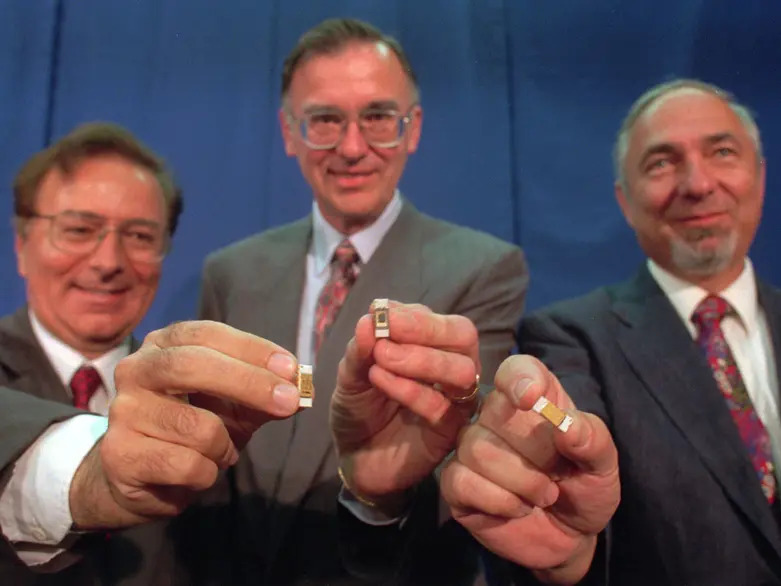
\includegraphics[scale = 0.25]{Graphics/faggin_hoff_mazor_-4004.jpg}
	\caption{Desde la izquierda, \emph{Federico Faggin}, \emph{Ted Hoff} y \emph{Stanley Mazor} con procesadores \textbf{Intel 4004}}
	\label{fig:10}
\end{figure}

\subsection{Intel 4004}
Este revolucionario \textbf{procesador}, del tamaño de la uña del dedo meñique, entregaba la misma potencia de cómputo que la primera
computadora electrónica construida en 1946, que llenó una habitación entera. El primer \textbf{microprocesador} \textbf{Intel 4004} se
fabricó en obleas de dos pulgadas, en comparación con las obleas de 12 pulgadas que se utilizan habitualmente en los productos actuales.
El \textbf {microprocesador} \textbf{Intel 4004} es único en el sentido de que es uno de los diseños de \textbf{microprocesador} más
pequeños que alguna vez entró en producción comercial. El \textbf{4004}  era un \textbf{microprocesador} de \textbf{4-bits}, alcanzaba una 
frecuencia de reloj máxima de 740 kHz. El ancho de línea del circuito (proceso de fabricación) del \textbf{microprocesador} \textbf{Intel 4004} 
era de 10 micrones o 10 000 nanómetros. En 1971 el \textbf{Intel 4004} contenía 2300 \textbf{transistores}. Para el 2010, un procesador \textbf{Intel Core} con matriz de procesamiento
de 32 nm y tecnología de \textbf{silicio} de puerta metálica de alta k de segunda generación contenía  560 millones de transistores. En comparación,
un cabello humano promedio tiene 100,000 nanómetros de ancho \brackcite{intel_4004,wikipedia_2022_intel_4004}.      

\begin{figure}[htb]
	\centering
	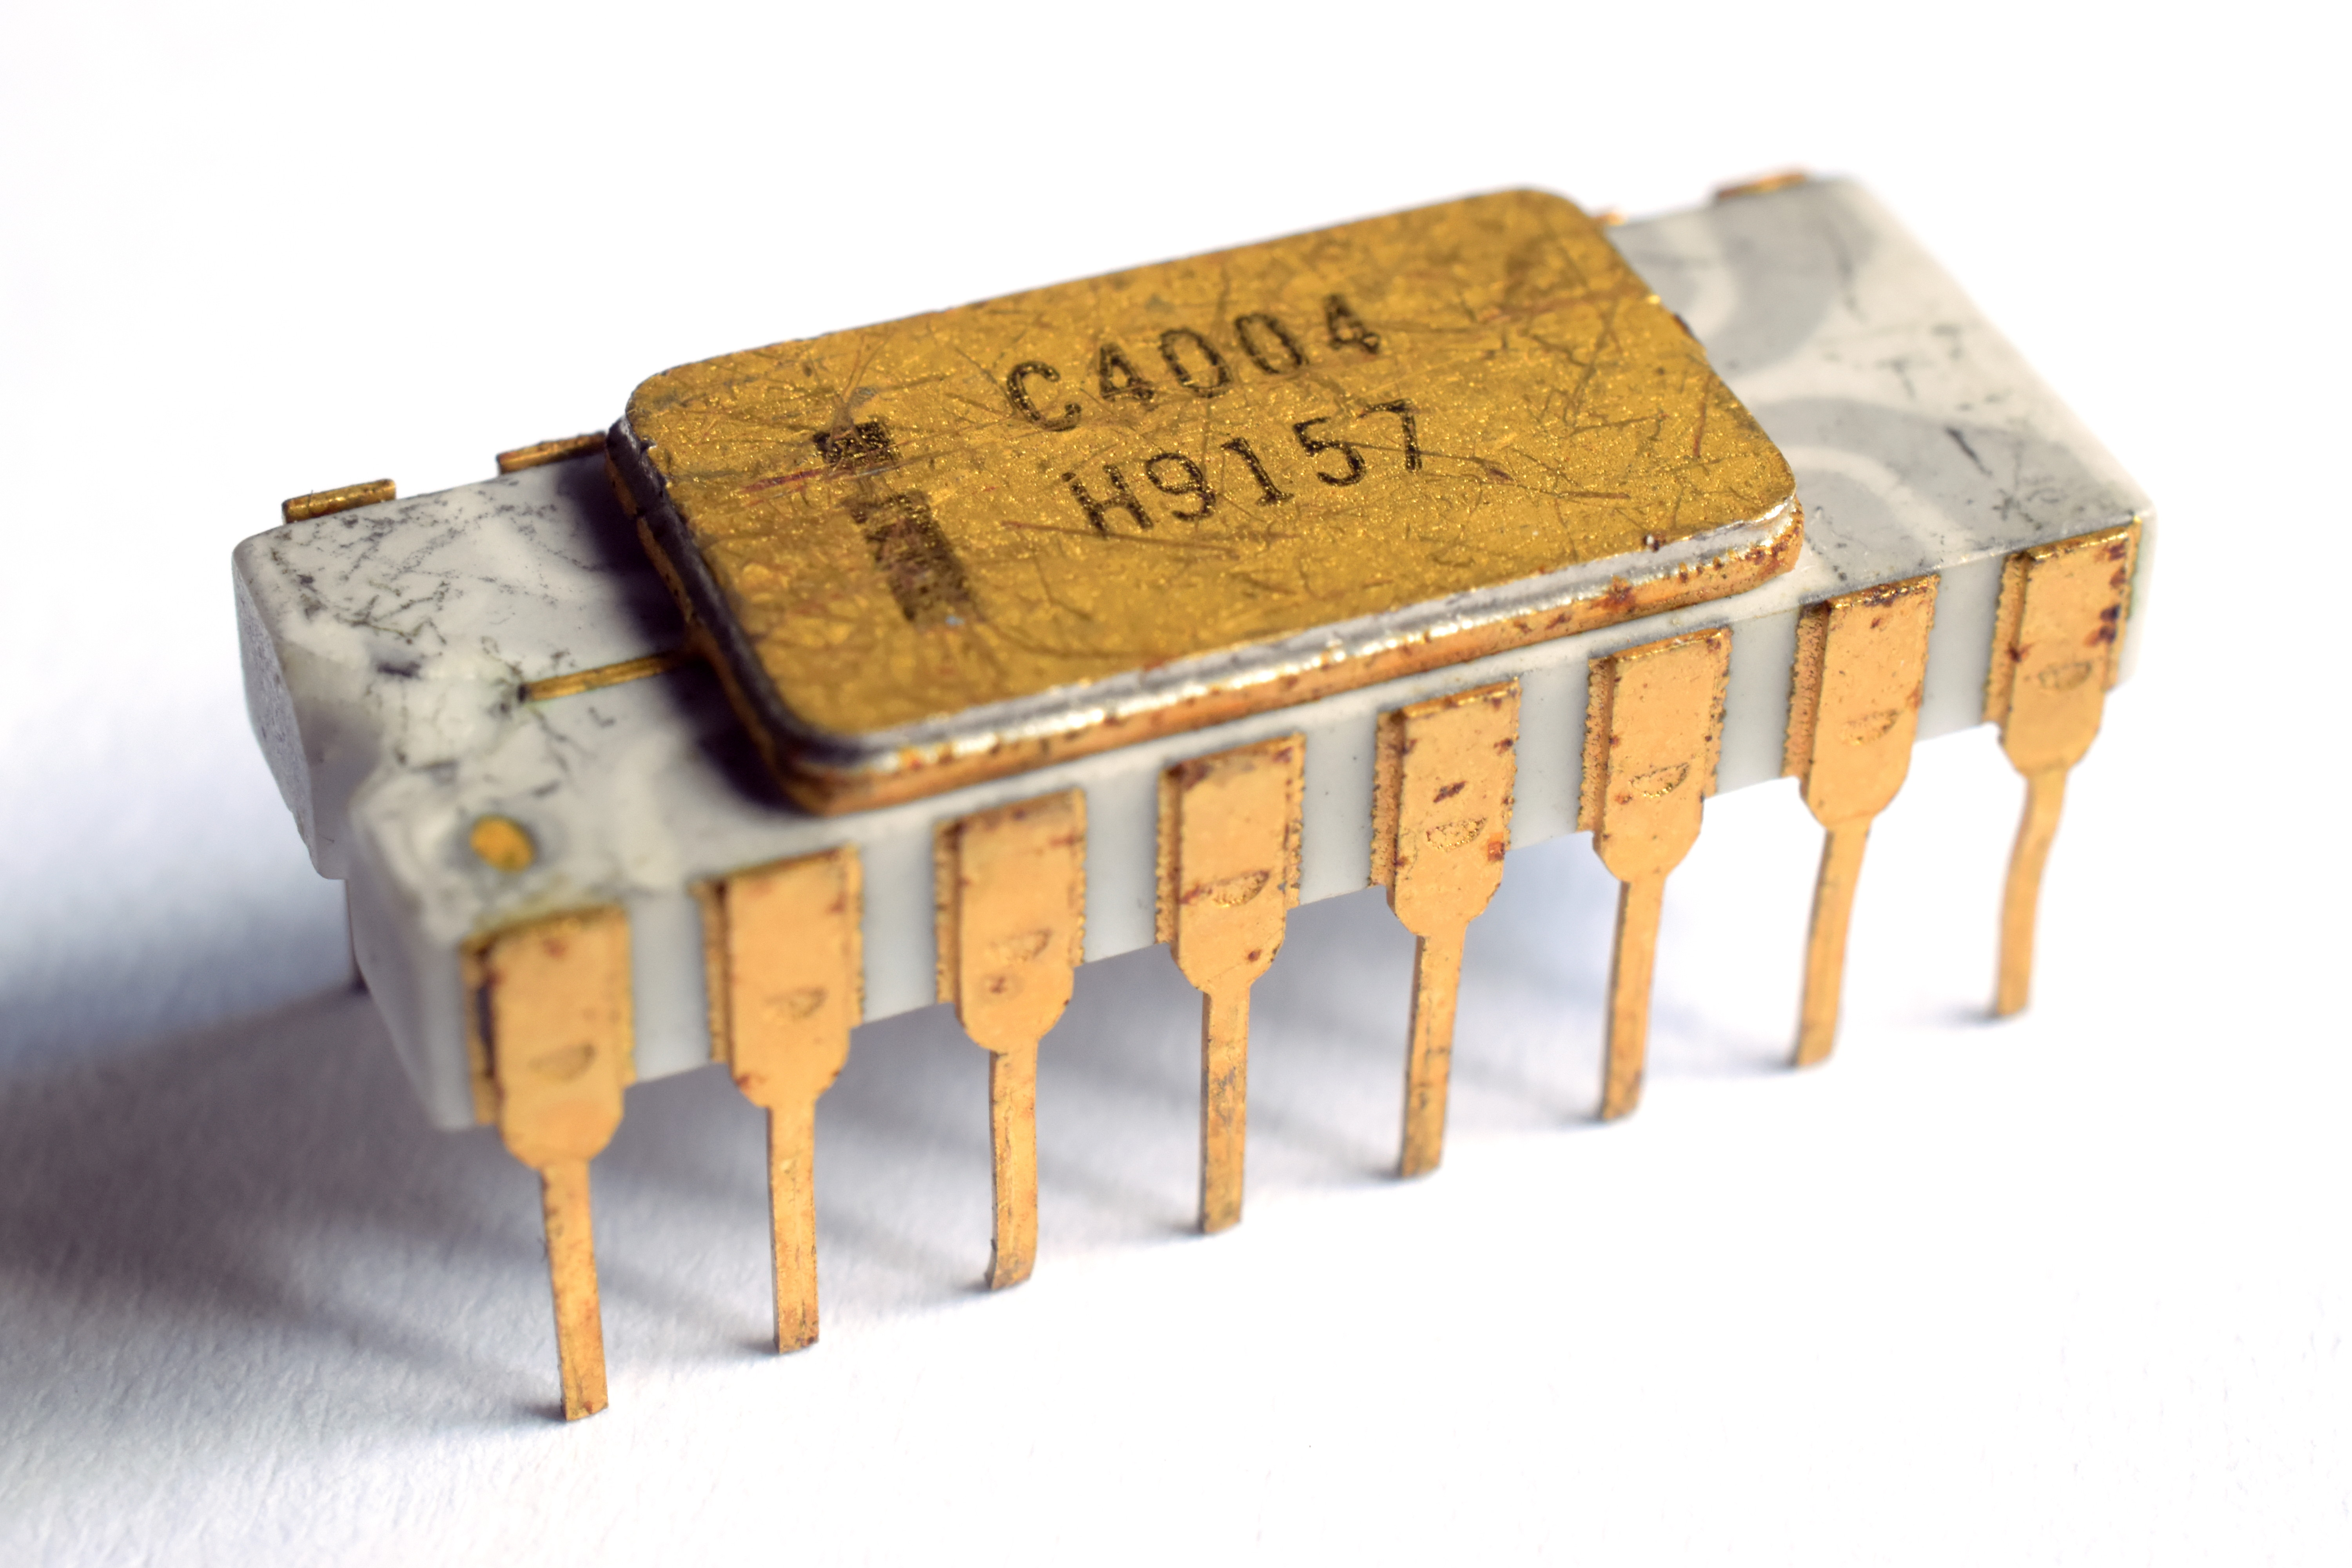
\includegraphics[scale = 0.15]{Graphics/Intel_C4004.jpg}
	\caption{Primer \textbf{microprocesador}: \textbf{Intel 4004}}
	\label{fig:12}
\end{figure}


\section{El arribo del primer microprocesador de 8-bits}
El \textbf{Intel 4004} fue seguido en 1972 por el \textbf{Intel 8008}, el primer \textbf{microprocesador} de 8 bits del mundo.
Sin embargo, el \textbf{8008} no fue una extensión del diseño del \textbf{4004}, sino la culminación de un proyecto de diseño separado
en \emph{Intel}, que surgió de un contrato con \emph{Computer Terminals Corporation}(\textbf{CTC}), por un \emph{chip} para
una terminal que estaban diseñando: el \textbf{Datapoint 2200}, los aspectos fundamentales del diseño no provinieron de \emph{Intel}
sino de \textbf{CTC}. El \textbf{8008} salió con 3.500 transistores, tenía un bus de datos de 8 bits y un bus de direcciones de 14 bits. Este
\textbf{micoprocesador} fue la base del famoso kit de computadora \textbf{"Mark-8"} \brackcite{wikipedia_2022_intel_8008, campbell-kelly_garcia-swartz_2015}.

\begin{figure}[htb]
	\centering
	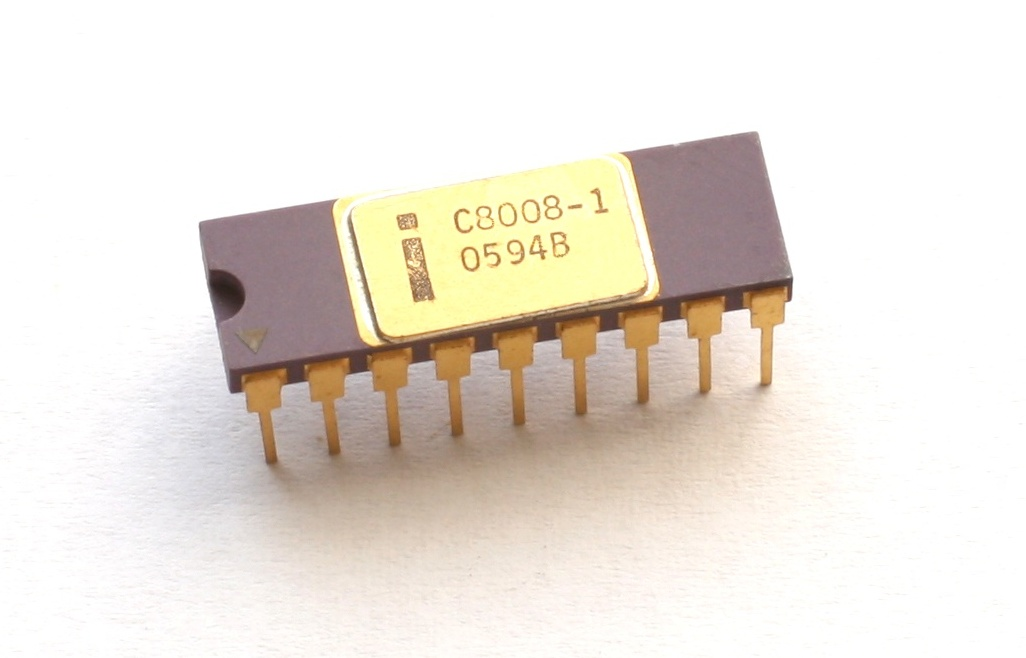
\includegraphics[scale = 0.15]{Graphics/Intel_C8008-1.jpg}
	\caption{\textbf{Microprocesador}  \textbf{Intel 8008}}
	\label{fig:13}
\end{figure}

\subsection{8080}
El  \textbf{Intel 8080} es el segundo \textbf{microprocesador} de 8 bits diseñado y fabricado por Intel. Apareció por primera vez en abril de
1974 y es una variante ampliada y mejorada del diseño anterior del \textbf{8008}, aunque sin compatibilidad binaria. La velocidad de reloj o
límite de frecuencia especificado inicialmente era de 2 MHz, con instrucciones comunes que usaban 4, 5, 7, 10 o 11 ciclos. Como resultado,
el \textbf{procesador} podía ejecutar varios cientos de miles de instrucciones por segundo. \emph{Federico Faggin} lo concibió y diseñó 
utilizando \textbf{MOS} de canal N de alto voltaje \brackcite{sexton_2018_history_of_intel_cpus,wikipedia_2022_Microprocesador,wikipedia_2022_microprocessor_chronology}.

\begin{figure}[htb]
	\centering
	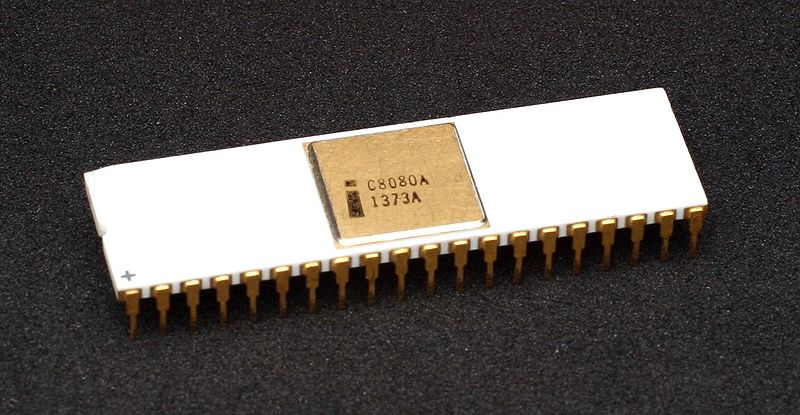
\includegraphics[scale = 0.2]{Graphics/8080_microprocessorr.jpg}
	\caption{\textbf{Microprocesador} \textbf{Intel 8080}}
	\label{fig:14}
\end{figure}

\section{El arribo de los 16 bits}
El primer \textbf{microprocesador} multichip de 16 bits fue el \textbf{IMP-16} de \emph{National Semiconductor}, presentado a principios de
1973. Una versión de 8 bits del conjunto de chips se introdujo en 1974 como \textbf{IMP-8}. Durante el mismo año, \emph{National} presentó
el primer \textbf{microprocesador} de un solo \emph{chip} de 16 bits, el \textbf{PACE}, seguido de una versión NMOS, el \textbf{INS8900}.
El primer \textbf{microprocesador} de 16 bits de un solo chip fue el \textbf{TMS 9900} de \emph{Texas Instruments}, presentado en 1976, que también
era compatible con su línea de minicomputadoras \textbf{TI-990}. \emph{Intel} produjo su primer \textbf{microprocesador} de 16 bits, el \textbf{8086},
en 1978. Era compatible con el \textbf{8080} y el \textbf{8085} (un derivado del \textbf{8080}) \brackcite{wikipedia_2022_Microprocesador,
staff_2021_microprocessor}.

\begin{figure}[htb]
	\centering
	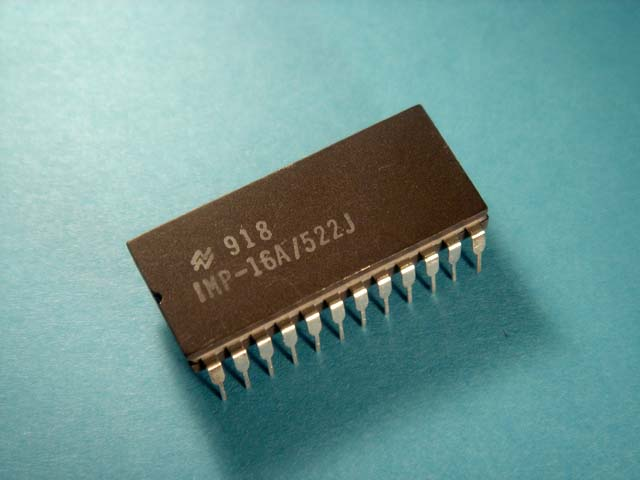
\includegraphics[scale = 0.2]{Graphics/NSIMP-16A.jpg}
	\caption{\textbf{Microprocesador} \textbf{IMP-16}}
	\label{fig:15}
\end{figure}

\section{8086: El comienzo de x86}
El primer \textbf{microprocesador} de 16 bits de \emph{Intel} fue el \textbf{8086}, que ayudó a mejorar considerablemente el rendimiento en comparación
con los diseños anteriores. Este \textbf{microprocesador} utilizaba la misma microarquitectura que los microprocesadores de 8 bits de \emph{Intel}
(\textbf{8008}, \textbf{8080} y \textbf{8085}). Esto permitió que los programas en lenguaje ensamblador escritos en 8 bits migraran sin
problemas. El \textbf{8086} no solo tenía una frecuencia más alta que la \textbf{8088}, sino que también empleaba un bus de datos externo
de 16 bits y una cola de precarga de 6 bytes más larga. También podía ejecutar tareas de 16 bits (aunque la mayoría del \emph{software} en
ese momento estaba diseñado para procesadores de 8 bits). El bus de direcciones se amplió a 20 bits, lo que permitió al \textbf{8086} acceder
a hasta 1 MB de memoria y, por lo tanto, aumentar el rendimiento. El \textbf{8086} también se convirtió en el primer \textbf{microprocesador} x86 y utilizó
la primera revisión del x86 ISA \brackcite{wikipedia_2022_x86_ISA}, en el que se han basado casi todos los procesadores creados por \emph{AMD}
o \emph{Intel} desde la introducción del \textbf{8086} \brackcite{wikipedia_2022_Microprocesador, sexton_2018_history_of_intel_cpus,  wikipedia_2022_intel_8086}.

\begin{figure}[htb]
	\centering
	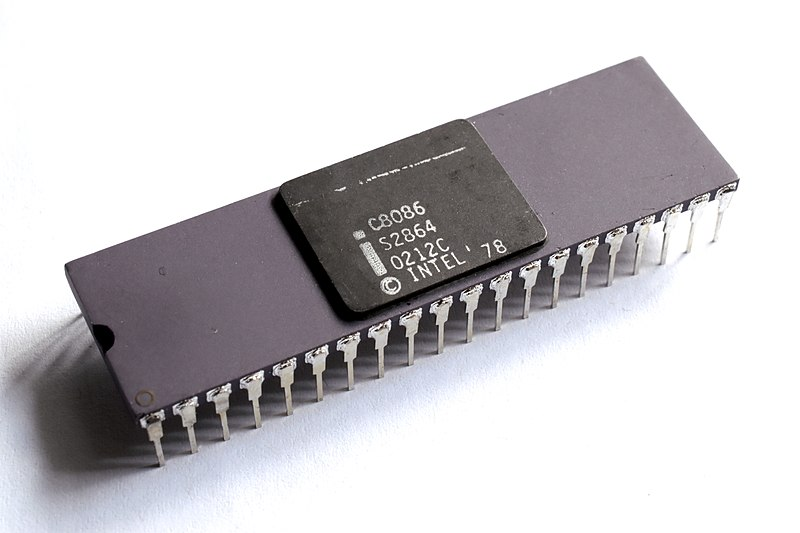
\includegraphics[scale = 0.2]{Graphics/Intel_C8086.jpg}
	\caption{\textbf{Microprocesador Intel 8086}}
	\label{fig:16}
\end{figure}

\section{El arribo de los 32 bits}
Los diseños de 16 bits solo habían estado en el mercado brevemente cuando comenzaron a aparecer implementaciones de 32 bits.
El más significativo de los diseños de  microprocesadores de 32 bits fue el \textbf{Motorola MC68000}, introducido en 1979. 
El \textbf{68k}, como se le conocía ampliamente, tenía  registros de 32 bits en su modelo de programación pero usaba rutas internas
de datos de 16 bits, tres unidades aritméticas-lógicas de 16 bits, y un bus de datos externo de 16 bits para reducir 
el conteo de pines. Soportaba externamente solo direcciones de 24 bits (internamente funcionaba con direcciones completas de 
32 bits). Los diseños de \textbf{Apple Lisa} y \textbf{Macintosh} utilizaron el \textbf{68k}, al igual que muchos otros diseños a
mediados de la década de 1980, incluidos \textbf{Atari ST} y \textbf{Commodore Amiga}. El primer \textbf{microprocesador} de 32 bits de
un solo \emph{chip} del mundo, con rutas de datos de 32 bits, buses de 32 bits y direcciones de 32 bits, fue el \textbf{AT\&T Bell Labs BELLMAC-32A},
con las primeras muestras en 1980 y la producción general en 1982. Después de la venta de \emph{AT} \& \emph{T} en 1984, pasó a llamarse \textbf{WE 32000}
(de \emph{Western Electric}) y tuvo dos generaciones posteriores, \textbf{WE 32100} y \textbf{WE 32200}. El primer microprocesador comercial de
un solo \emph{chip} de 32 bits disponible en el mercado fue el \textbf{HP FOCUS}. El primer \textbf{microprocesador} de 32 bits de \emph{Intel} 
fue el \textbf{iAPX 432}, que se introdujo en 1981, pero no fue un éxito comercial. Tenía una arquitectura orientada a objetos basada en capacidades avanzadas,
pero un rendimiento deficiente en comparación con las arquitecturas contemporáneas, como la \textbf{80286} de \emph{Intel}(introducida en 1982),
que era casi cuatro veces más rápida en las pruebas de referencia típicas. Este pobre rendimiento del \textbf{iAPX 432} se debieron en parte a un
compilador de Ada apresurado y, por lo tanto, subóptimo \brackcite{wikipedia_2022_Microprocesador,wikipedia_2022_motorola_68k}.

\begin{figure}[htb]
	\centering
	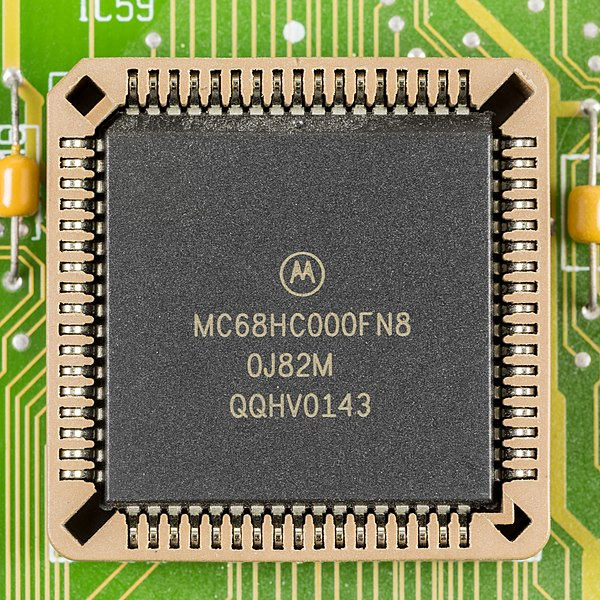
\includegraphics[scale = 0.15]{Graphics/Motorola_MC68HC000FN8-0695.jpg}
	\caption{\textbf{Microprocesador Motorola 68K}}
	\label{fig:17}
\end{figure}

\subsection{80386: x86 se convierte a 32-bit}
El primer \textbf{microprocesador} x86 de 32 bits de \emph{Intel} fue el \textbf{80386}(renombrado más tarde como \textbf{i386}), lanzado en 1985. Una ventaja clave que 
tenía este \textbf{microprocesador} era su bus de direcciones de 32 bits que le permitía admitir hasta 4 GB de memoria del sistema. Aunque esto era mucho 
más de lo que nadie estaba usando en ese momento, las limitaciones de \textbf{RAM} a menudo perjudicaban el rendimiento de los procesadores x86 anteriores y de la competencia. 
\brackcite{sexton_2018_history_of_intel_cpus,wikipedia_2022_intel_i386}.

\begin{figure}[htb]
	\centering
	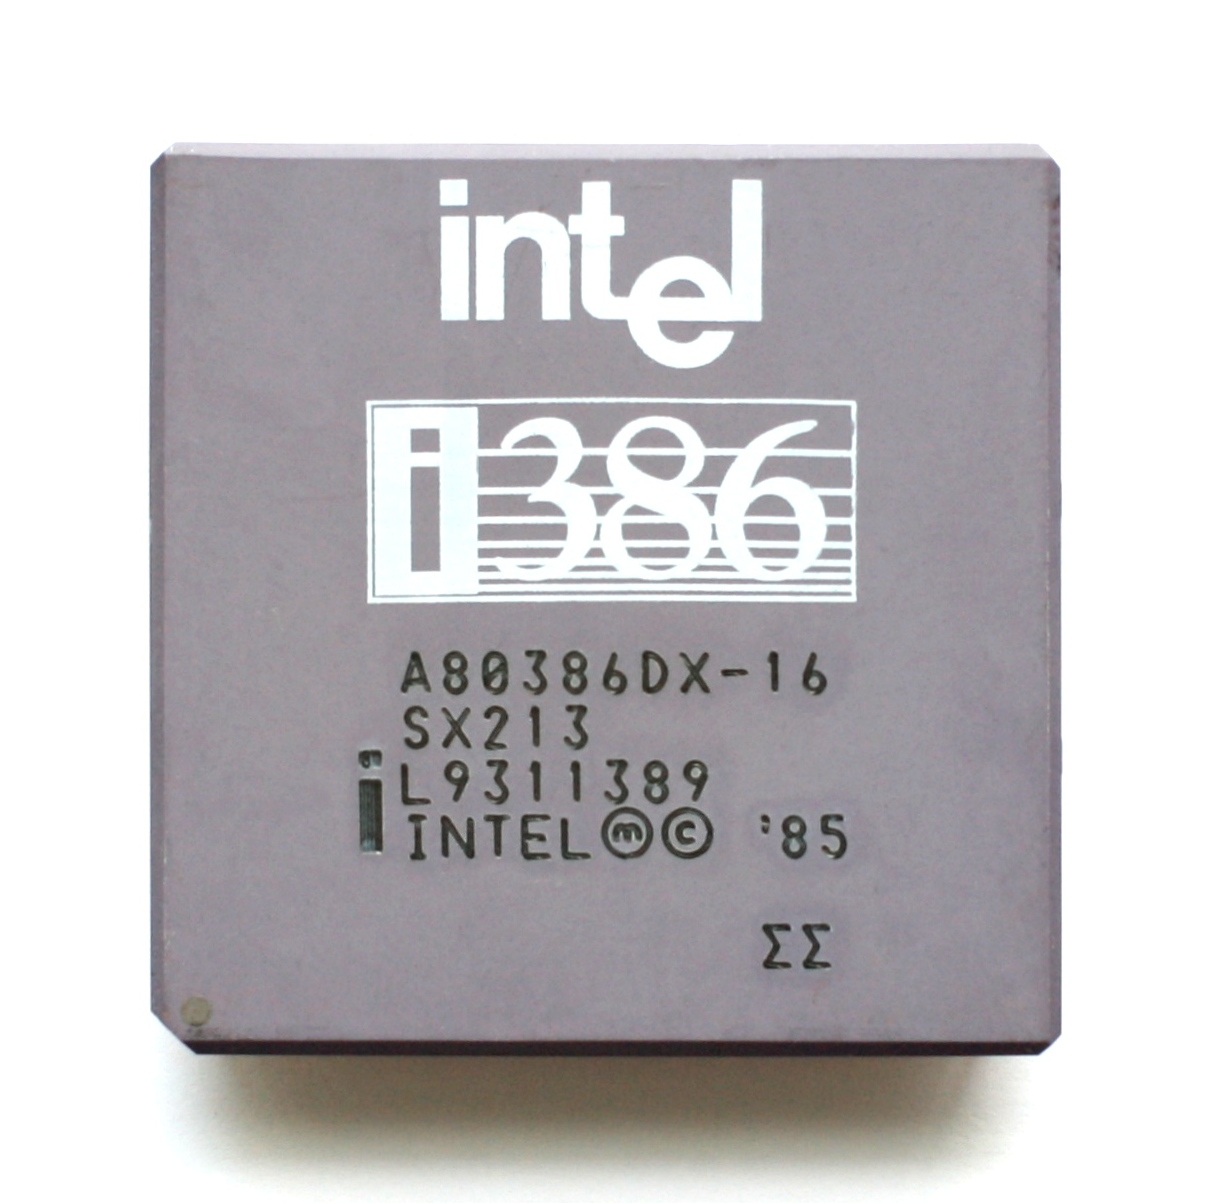
\includegraphics[scale = 0.1]{Graphics/Intel_i386DX.jpg}
	\caption{\textbf{Microprocesador Intel i386}}
	\label{fig:18}
\end{figure}
\newpage

\section{El arribo de los 64 bits}
Antes que se introdujeran los primeros microprocesadores de 64 bits destinados a las computadoras personales, desde principios de la década de
1990 se utilizaron diseños de microprocesadores de 64 bits en varios mercados. En 1991 \textbf{MIPS Computer Systems} produce el primer \textbf
{microprocesador} de 64 bits, el \textbf{R4000}, que implementa la arquitectura \textbf{MIPS III}, la tercera revisión de su arquitectura \textbf{MIPS}.
El \textbf{R4000} se utilizó en estaciones de trabajo de gráficos SGI. En 1996 la compañía nipona de videojuegos \emph{Nintendo} introduce la consola de
videojuegos \textbf{Nintendo 64}, que utiliza el \textbf{microprocesador VR4300} de 64 bits, construido alrededor de una variante de bajo costo del
\textbf{MIPS R4000}. En 1998 \emph{IBM} lanza la línea \textbf{POWER3} de microprocesadores de 64 bits 
\brackcite{wikipedia_2022_Microprocesador,wikipedia_2022_microprocessor_chronology, wikipedia_2022_r4000, wikipedia_2022_nintendo64_specs}. 

\subsection{La llegada de los 64 bits a las computadoras personales}
En septiembre de 2003 \emph{AMD} introduce la arquitectura de 64 bits retrocompatible con x86, x86-64 (también llamada \textbf{AMD64}). La línea
de procesadores \textbf{Opteron} y \textbf{Athlon 64}, fue la primera basada en la arquitectura \textbf{AMD64}. En 2004 \emph{Intel} introduce la
arquitectura \textbf{EM64T}(luego fue renombrada a \textbf{Intel 64}), que es una versión de 64 bits de la arquitectura x86. La primera línea
de procesadores basados en \textbf{EM64T} fue la línea \textbf{Pentium 4}. Ambas versiones pueden ejecutar aplicaciones heredadas de 32 bits sin ninguna
penalización en el rendimiento, así como el nuevo software de 64 bits \brackcite{wikipedia_2022_Microprocesador}.

\begin{figure}[htb]
	\centering
	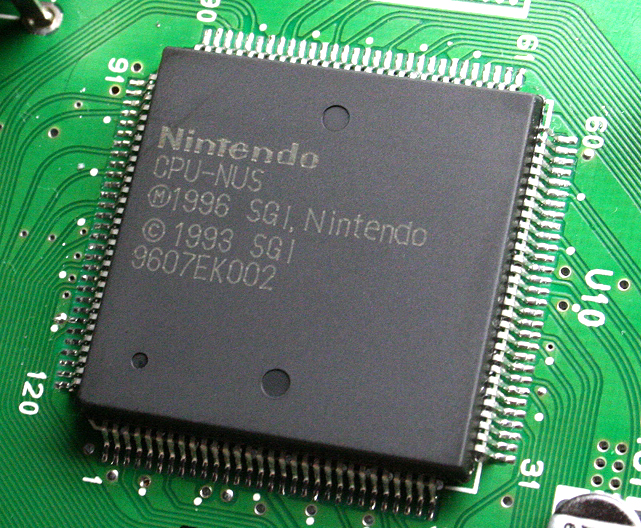
\includegraphics[scale = 0.15]{Graphics/CPU-NUS_01-Nintendo64.jpg}
	\caption{\textbf{Microprocesador VR4300} de la \textbf{Nintendo 64}}
	\label{fig:19}
\end{figure}

\begin{figure}[htb]
	\centering
	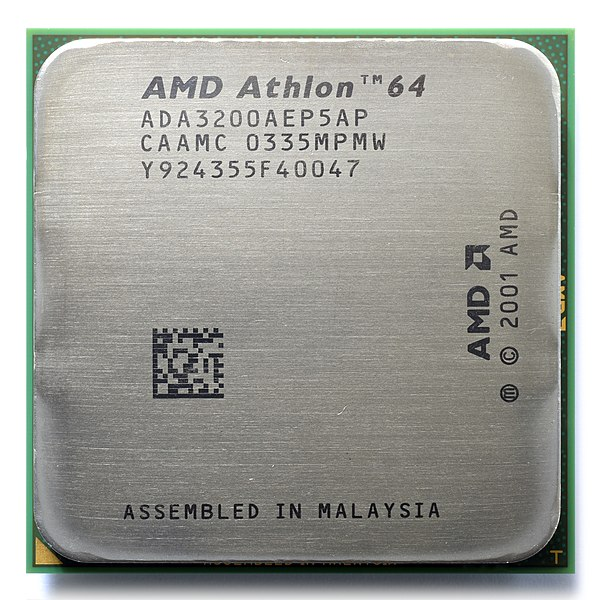
\includegraphics[scale = 0.15]{Graphics/AMD_Athlon_64_3200+_ADA3200AEP5AP.jpg}
	\caption{\textbf{Microprocesador AMD Athlon 64 3200}}
	\label{fig:20}
\end{figure}
\newpage

\section{Intel: el camino hacia los Intel Core}
\emph{Intel Corporation} es una corporación multinacional estadounidense y una empresa de tecnología con sede en \emph{Santa Clara, California}. 
Es el fabricante de chips semiconductores más grande del mundo por ingresos y es uno de los desarrolladores de la serie x86 
de conjuntos de instrucciones x86 \brackcite{wikipedia_2022_x86_ISA}, los conjuntos de instrucciones que se encuentran en la mayoría de las 
computadoras personales. Muchos de sus productos como el \textbf{4004} o el \textbf{8086}, vistos en las secciones anteriores, ocupan un lugar especial 
en la historia de los microprocesadores. A continuación veremos a otros de los microprocesadores y las arquitecturas que convirtieron 
a este gigante de los semiconductores en lo que es hoy en día.

\subsection{80186 y 80188}
\emph{Intel} siguió al \textbf{8086} con  otros procesadores, los cuales usaban una arquitectura similar de 16 bits. El primero fue \textbf{80186}, 
destinado a aplicaciones integradas. Para facilitar esto, \emph{Intel} integró varias piezas de hardware que normalmente se encuentran en la 
placa base (\emph{motherboard}) en la \textbf{CPU}, incluido el generador de reloj, el controlador de interrupción y el temporizador. El \textbf{80188}, 
orientado al presupuesto, contenía de manera similar varias piezas de hardware integradas en el \textbf{procesador}. Pero al igual que el \textbf{8088}, 
su bus de datos se redujo a la mitad \brackcite{sexton_2018_history_of_intel_cpus}.

\subsection{80286: más memoria, más rendimiento}
El \textbf{80286}(también comercializado como \textbf{iAPX 286} y a menudo llamado \textbf{Intel 286}) se lanzó en 1982, el mismo año que el \textbf{80186} y tenía
características casi idénticas, pero ampliaba el bus de direcciones a 24 bits, lo que permitía al \textbf{microprocesador} acceder a hasta 16 MB de memoria.
El \textbf{80286} usó aproximadamente 134,000 transistores. \brackcite{sexton_2018_history_of_intel_cpus,wikipedia_2022_80286, wikipedia_2022_80286}.

\subsection{80486: integrando la FPU}
El \textbf{80486}(\textbf{i486}) de \emph{Intel} fue otro paso importante en términos de rendimiento. La clave de su éxito fue una integración más estrecha de los componentes 
en la \textbf{CPU}. El \textbf{80486} fue la primera \textbf{CPU} x86 en contener caché L1. Los primeros modelos \textbf{80486} venían con 8 KB en matriz y se grabaron en un proceso de 1000 nm.
\emph{Intel} también incorporó la \textbf{FPU}(unidad de punto flotante diseñada especialmente para llevar a cabo operaciones con números de punto flotante) a la \textbf{CPU}, que hasta ese 
momento había sido una unidad de procesamiento funcional independiente. Al mover estas piezas de \emph{hardware} al procesador, la latencia entre ellas se redujo 
drásticamente. El \textbf{80486} también usó una interfaz FSB(front-side bus)\brackcite{wikipedia_2022_front_side_bus} más rápida para aumentar el ancho de banda, y el núcleo 
tenía varios ajustes para impulsar el \textbf{IPC}(Del inglés \emph{instructions per clock} es la cantidad de instrucciones que es 
capaz de ejecutar por cada ciclo de reloj el microprocesador). Estos cambios aumentaron significativamente el rendimiento del \textbf{80486} 
\brackcite{sexton_2018_history_of_intel_cpus,wikipedia_2022_intel_80486}. 

\begin{figure}[htb]
	\centering
	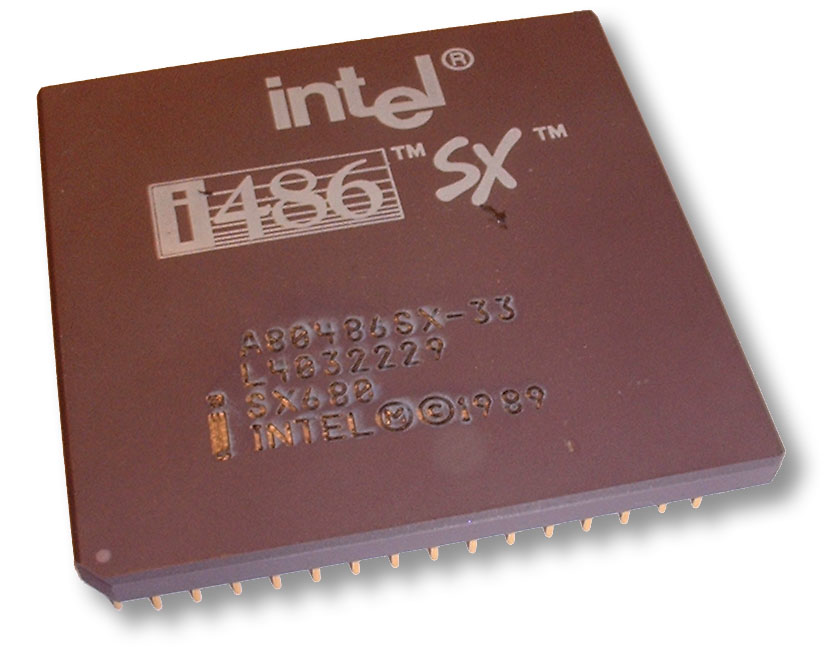
\includegraphics[scale = 0.15]{Graphics/Intel_80486sx.jpg}
	\caption{\textbf{Microprocesador Intel i486}}
	\label{fig:21}
\end{figure}

\subsection{Pentium}

El \textbf{Pentium} surgió en 1993 como el primer microprocesador \emph{Intel x86} que no seguía el sistema numérico 80x86. Internamente, el \textbf{Pentium} utilizó 
la arquitectura \textbf{P5}, que fue el primer diseño superescalar \emph{x86} de \emph{Intel}. Aunque el \textbf{Pentium} fue generalmente más rápido que 
el \textbf{80486} en todos los sentidos, su característica más destacada fue una \textbf{FPU} sustancialmente mejorada. La \textbf{FPU} del \textbf{Pentium} original 
era hasta 10 veces más rápida que la unidad antigua del \textbf{80486}. Esto se convirtió en una característica aún más significativa en años posteriores cuando \emph{Intel} 
lanzó el \textbf{Pentium MMX}. Este microprocesador tenía la misma arquitectura que el \textbf{Pentium} original, pero incluía soporte para el nuevo conjunto de instrucciones 
\textbf{MMX SIMD} de \emph{Intel} que podría aumentar drásticamente el rendimiento. \emph{Intel} también aumentó el tamaño de caché L1 en sus procesadores \textbf{Pentium} en relación con el \textbf{80486}. 
Los \textbf{Pentium} iniciales contenían 16 KB, mientras que el \textbf{Pentium MMX} subió a 32 KB. Naturalmente, estos procesadores también funcionaron a velocidades de reloj más altas. 
\emph{Intel} planeó seguir rápidamente al \textbf{Pentium} con el \textbf{Pentium Pro} basado en su arquitectura \textbf{P6}, pero se encontró con dificultades técnicas. El \textbf{Pentium Pro} 
fue considerablemente más rápido que el \textbf{Pentium} en operaciones de 32 \emph{bits}, gracias a su diseño \emph{out-of-order}(paradigma en el que el microprocesador ejecuta 
instrucciones en un orden regido por la disponibilidad de datos de entrada y unidades de ejecución, en lugar de por su orden original en un programa)\brackcite{wikipedia_2022_out_of_order}. En 1997 cuando con el lanzamiento de 
\textbf{Pentium II} se logró superar casi todos los aspectos negativos del \textbf{Pentium Pro}. Su arquitectura subyacente era similar a la del \textbf{Pentium Pro}, 
y continuó usando un \emph{papeline} de 14 etapas con varias mejoras en el núcleo para mejorar el textbf{IPC}. \emph{Intel} planeó continuar luego  del \textbf{Pentium II} con un procesador basado en su arquitectura \emph{Netburst}, 
pero aún no estaba listo. En cambio, \emph{Intel} volvió a impulsar la arquitectura \textbf{P6} con \textbf{Pentium III}. Gracias a un \emph{pipeline} actualizado y a un 
aumento en la velocidad del reloj(el \textbf{Intel Pentium III-T Tualatin-256} llegó a alcanzar los 1.13GHz), los procesadores \textbf{Pentium III} superaron a sus 
homólogos \textbf{Pentium II} \brackcite{wikipedia_2022_pentiumIII,wikipedia_2022_pentium,sexton_2018_history_of_intel_cpus}.\\ En 2000, la arquitectura \emph{Netburts} de \emph{Intel} finalmente estuvo lista y se puso en producción como \textbf{Pentium 4}. 
Los microprocesadores de \emph{Intel} llevarían esta arquitecura durante los próximos seis años. La primera implementación de esta arquitecura fue nombrada como 
\emph{Willamette}, en la cual se basaron los \textbf{Pentium 4} durante los primeros dos años. Sin embargo, este fue un momento difícil para \emph{Intel}, y el chip luchó para 
superar al \textbf{Pentium III}. \emph{Netburts} permitió frecuencias significativamente más altas y \emph{Willamette} logró alcanzar los 2 GHz, pero el \textbf{Pentium III} 
a 1,4 GHz fue aún más rápido en algunas tareas. La situación mejoró con el diseño a 130 nm de \emph{Intel} conocido como \emph{Northwood}, el cual  amplió la frecuencia 
de reloj hasta los 3,2 GHz y duplicó la memoria caché L2 de 256 KB a 512 KB. \emph{Northwood} se desempeñó significativamente mejor y fue muy competitivo frente a los microprocesadores 
de \emph{AMD} de esa época.
En los modelos de gama alta, \emph{Intel} también introdujo su tecnología \textbf{Hyper-Threading}(innovación de hardware que permite que se ejecuten varios subprocesos en cada núcleo, 
lo que significa que se puede hacer más trabajo en paralelo)\brackcite{WhatIsHy83:online} para mejorar la utilización de recursos en entornos que 
enfatizaban la multitarea. \textbf{Hyper-Threading} no fue tan beneficioso en \emph{Northwood} como lo es en los procesadores \textbf{Core i7} actuales, 
pero aumentó el rendimiento en algunos puntos porcentuales.
\emph{Northwood} llevó la arquitectura \emph{Netburts} desde 2002 hasta 2004, después de lo cual \emph{Intel} lanzó \emph{Prescott} con numerosas mejoras. 
Usó un proceso de fabricación de 90 nm que permitió a \emph{Intel} aumentar la caché L2 a 1 MB.  \emph{Prescott} tenía un ancho de banda significativamente mayor que \emph{Northwood}, 
lo cual fue vital para aumentar el rendimiento de \emph{Netburts} \brackcite{sexton_2018_history_of_intel_cpus, wikipedia_2022_pentium_4}.


\begin{figure}[htb]
	\centering
	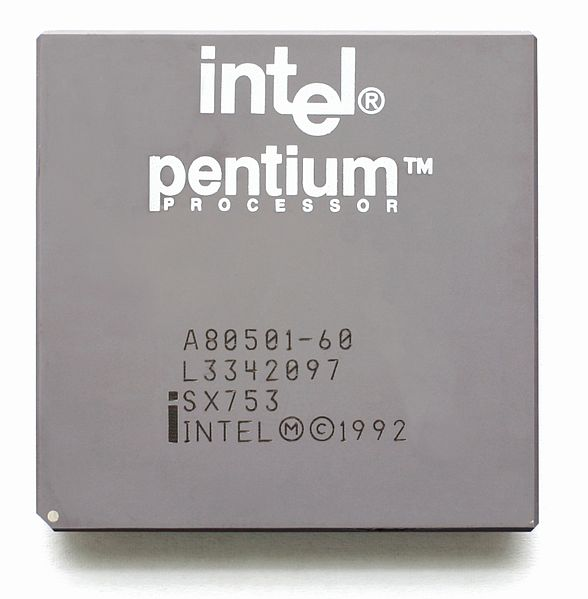
\includegraphics[scale = 0.15]{Graphics/Intel_Pentium_P5.jpg}
	\caption{\textbf{Microprocesador Intel Pentium P5}}
	\label{fig:22}
\end{figure}

\begin{figure}[htb]
	\centering
	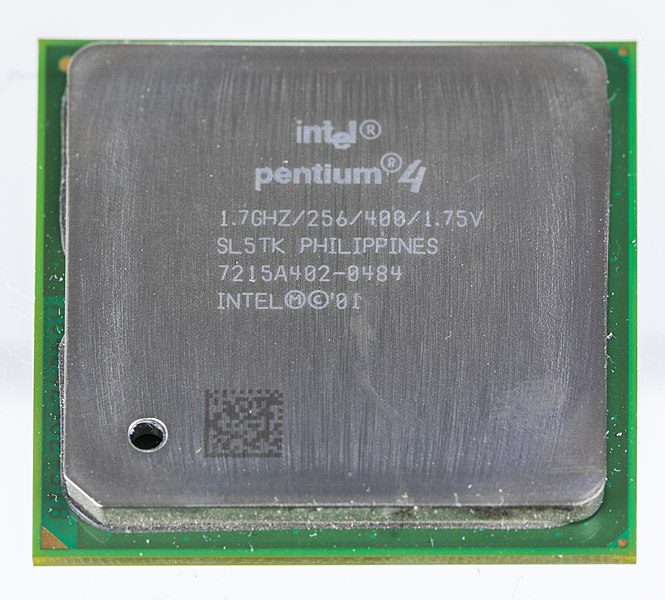
\includegraphics[scale = 0.15]{Graphics/Pentium_4_-_SL5TK-3056.jpg}
	\caption{\textbf{Microprocesador Intel Pentium 4 Willamette}}
	\label{fig:23}
\end{figure}

\subsection{Intel Core 2}
\emph{Intel} finalmente renunció a su arquitectura \emph{Netburst}. La empresa se dio cuenta de que \textbf{P6} aún era viable y capaz de ser eficiente y brindar 
un excelente rendimiento. Reelaboró la arquitectura con su diseño \emph{Core}. El 27 de julio de 2006 se introdujo la línea de procesadores \textbf{Core 2}.
\textbf{Intel Core 2} abarcaba una gama de microprocesadores \emph{Intel} de consumo de 64 bits x86-64 de uno, dos y cuatro 
núcleos basados en la microarquitectura \textbf{Core}. Los modelos de uno y dos núcleos son de un solo \emph{die}(parte donde se encuentra 
todo el circuito y los componentes internos del microprocesador), mientras que los modelos de cuatro núcleos comprenden dos \emph{dies}, cada una con dos núcleos, 
empaquetados en un módulo de varios chip(MCM). El tamaño de la memoria caché  L2 de los \textbf{Core 2} iba desde los 512 KB a los 
12 MB \brackcite{wikipedia_2022_intel_core_2, sexton_2018_history_of_intel_cpus}.

\begin{figure}[htb]
	\centering
	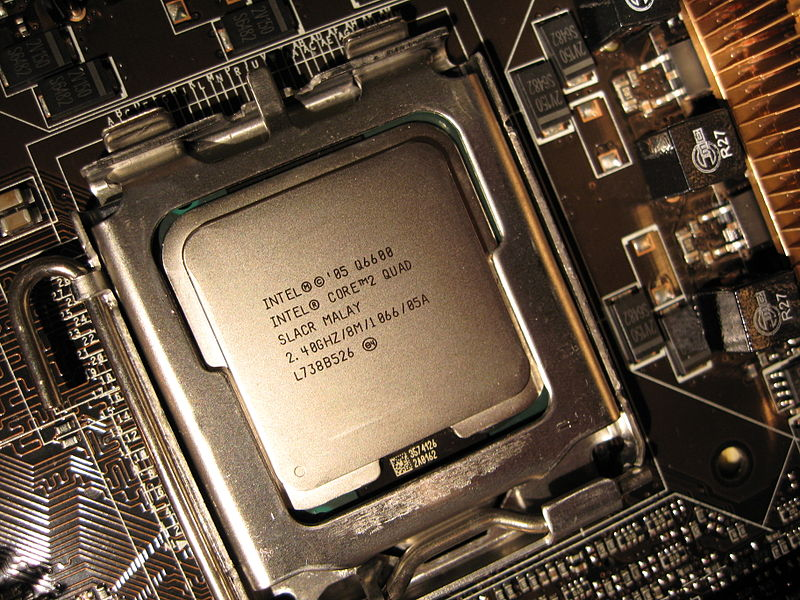
\includegraphics[scale = 0.8]{Graphics/IntelCore_2_Q6600.jpeg}
	\caption{\textbf{Microprocesador} de 4 núcleos  \textbf{ Intel Core 2 QuadQ6600} (\textbf{Intel Core 2})}
	\label{fig:24}
\end{figure}
\newpage

\subsection{Intel Core: la llegada de los i3, i5, i7}
Con el mercado de procesadores en un estado altamente competitivo, \emph{Intel} no pudo darse el lujo de quedarse quieto por mucho tiempo. 
Por lo tanto, modificó la arquitectura \emph{Core} para crear \emph{Nehalem}, que agregaba numerosas mejoras. El controlador de caché se rediseñó y 
la caché L2 se redujo a 256 KB por núcleo. Sin embargo, esto no afectó el rendimiento, ya que \emph{Intel} agregó entre 4 y 12 MB de caché L3 
compartidos entre todos los núcleos. Las \textbf{CPU} basadas en \emph{Nehalem} aparecieron entre uno y cuatro núcleos. La última gran 
ventaja que tuvo \emph{Nehalem} sobre la arquitectura \emph{Core} fue que marcó el regreso de la tecnología \textbf{Hyper-Threading}. Gracias a esta y 
muchas otras mejoras, \emph{Nehalem} pudo funcionar hasta el doble de rápido que los procesadores \textbf{Core 2} en cargas de trabajo con muchos 
subprocesos. \emph{Nehalem} funcionó a frecuencias de reloj comparables a \textbf{Core 2} y tenía un proceso de fabriación de 45nm. 
\emph{Nehalem} también fue el primer procesador de Intel en implementar \textbf{Turbo Boost} (característica que permite aumentar automáticamente la frecuencia 
de reloj cuando el sistema operativo solicita un estado de mayor rendimiento del \textbf{microprocesador}). Aunque el reloj base del procesador \emph{Nehalem} más rápido 
alcanzó un máximo de 3,33 GHz, podría operar a 3,6 GHz por períodos cortos gracias a esta nueva tecnología. La última gran ventaja que tuvo 
\emph{Nehalem} sobre la arquitectura \emph{Core 2} fue que marcó el regreso de la tecnología \textbf{Hyper-Threading}. 
Gracias a esta y muchas otras mejoras, \emph{Nehalem} pudo funcionar hasta el doble de rápido que los procesadores \textbf{Core 2} en cargas de trabajo con 
muchos subprocesos. \emph{Intel} vendió las \textbf{CPU} \emph{Nehalem} bajo las marcas \textbf{Celeron}, \textbf{Pentium},\textbf{Core i3}, \textbf{Core i5}, 
\textbf{Core i7} y \textbf{Xeon} \brackcite{sexton_2018_history_of_intel_cpus}.\\

\begin{figure}[htb]
	\centering
	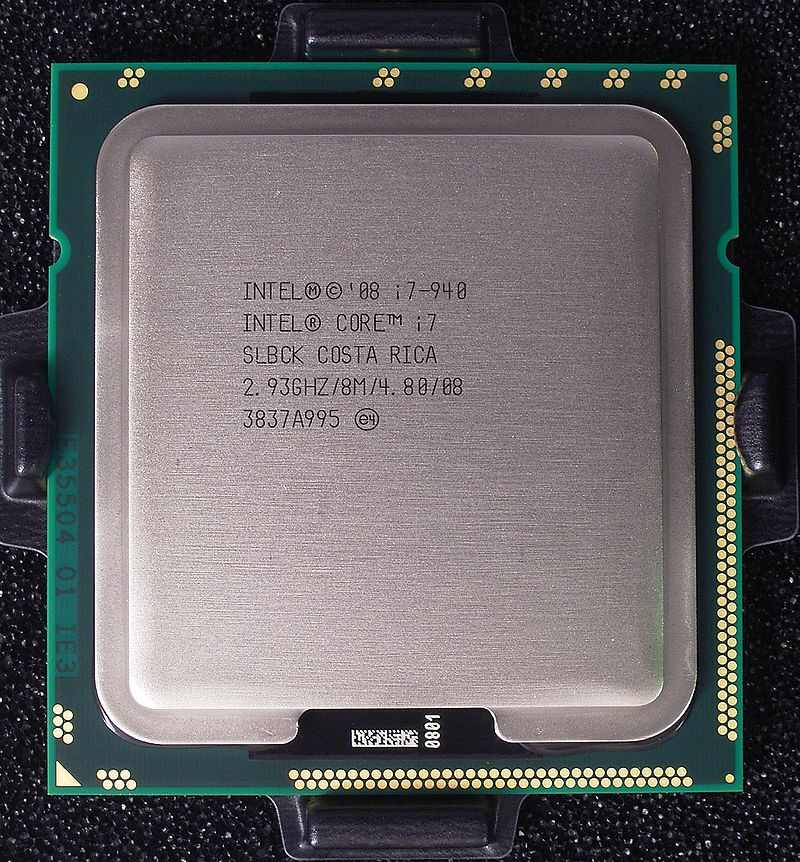
\includegraphics[scale = 0.2]{Graphics/Intel_core_i7_940_top_R7309478_wp.jpg}
	\caption{\textbf{Micropocesador Intel Core i7 940} basado \textbf{Nehalem}}
	\label{fig:25}
\end{figure}

La segunda, tercera, cuarta, quinta, sexta y séptima generación de los \emph{Intel Core} dieron un salto significativo en rendimiento, mejorando
el \textbf{IPC}, subiendo la frecuencia de reloj,  con   procesos de fabricación  más eficientes que llegaron hasta los 14 nm en la sexta y séptima generación.
Aumentaron la memoria caché, principalmente la L3(hasta 8MB compartidos en la séptima generación). Se mejoraron los gráficos integrados y se introdujeron 
compatibilidad con nuevas tecnologías como \textbf{Intel Optane} y \textbf{Thunderbolt 3} \brackcite{sexton_2018_history_of_intel_cpus,wikipedia_2022_intel_core}.  \\
Con la octava generación (\emph{Coffee Lake}), lanzada en 2017 se añadieron más núcleos. Se introdujeron microprocesadores \textbf{Core i5} y \textbf{Core i7} 
con seis núcleos (junto con \textbf{Hyper-Threading} en el caso de los i7) y microprocesadores Core i3 con cuatro núcleos y sin \textbf{Hyper-Threading}
\brackcite{sexton_2018_history_of_intel_cpus,wikipedia_2022_cofee_lake}.
La novena generación, lanzada en 2018 fue un refrescamiento de \emph{Coffe Lake}. Las principales diferencias con respecto a la 
octava generación \brackcite{sexton_2018_history_of_intel_cpus,wikipedia_2022_cofee_lake} (además del aumento de frecuencia del reloj) son:
\begin{itemize}
	\item Las \textbf{Core i7} pasan a tener 8/8 núcleos/hilos en comparación con los 6/12 que tenía los \textbf{Core i7} de octava generación.
	\item Los \textbf{Core i3} están equipados con tecnología \textbf{Turbo Boost}. 	
\end{itemize}

Con la décima y oncena generación(\emph{Comet Lake} y \emph{Rocket Lake} respectivamente) los \textbf{Core i7} pasaron a tener 8 núcleos/16 hilos mientras 
los \textbf{Core i5} pasaron a tener 6 núcleos/12 hilos. Estas dos generaciones representaron una ligera mejora a \emph{Coffe Lake} 
\brackcite{wikipedia_2022_comet_lake,wikipedia_2022_intel_core,wikipedia_2022_rocket_lake}.

\subsection{Alder Lake: la nueva arquitecura híbrida}

\emph{Intel} anunció oficialmente la decimosegunda generación de los procesadores \textbf{Intel Core} (\emph{Alder Lake}) en 2021, 
basados en una arquitectura híbrida que utiliza núcleos de rendimiento  y núcleos eficientes.

Por primera vez \emph{Intel} ha apostado en su gama principal de procesadores por el uso de dos tipos de núcleo de diferente 
rendimiento y consumo para acelerar las tareas del procesador:

\begin{itemize}
	\item Los \textbf{P-Cores} (\emph{Golden Cove}) son núcleos de gran tamaño y que ofrecen un gran rendimiento, pero a cambio de ser menos eficientes energéticamente.
	\item Los \textbf{E-Cores} (\emph{Gracemont}) son núcleos de menor tamaño, lo que le permite a \emph{Intel} colocar una mayor cantidad en un mismo espacio y 
	tienen menor consumo energético.
\end{itemize}


Dependiendo del modelo de \textbf{Intel Core 12} la cantidad de \textbf{P-Cores} y \textbf{E-Cores} varía, pero ambos trabajan al unísono y de manera coordinada. 
Para esto último hacen uso de una caché de 30 MB de tercer nivel(L3), la cual no solo le da acceso al mismo espacio de memoria 
a ambos tipos de núcleos, sino que además les permite trabajar conjuntamente en la ejecución de los procesos a ejecutar \brackcite{wikipedia_2022_alder_lake, roca_2021_alder_lake}.

\begin{figure}[htb]
	\centering
	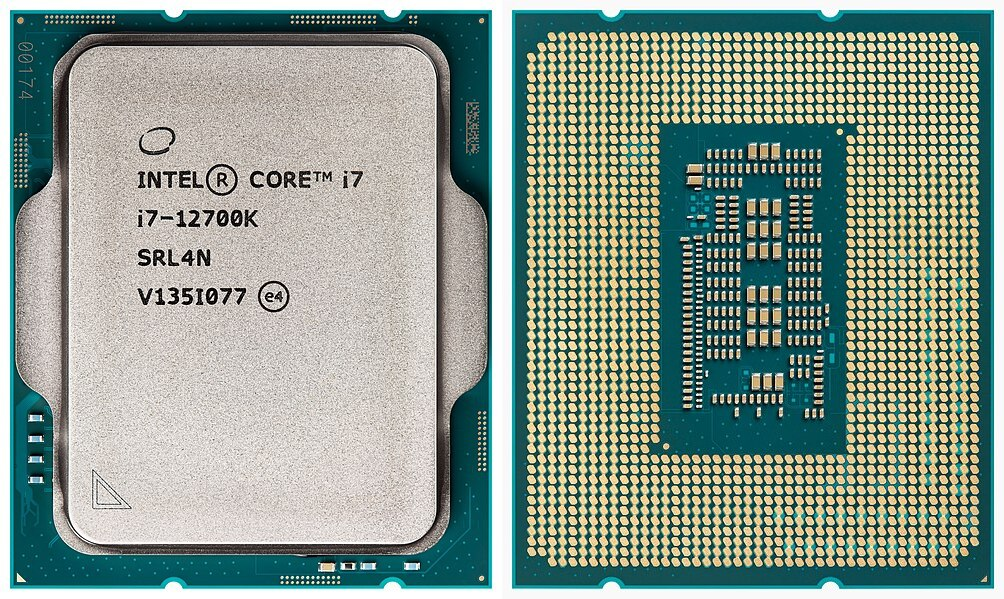
\includegraphics[scale = 0.2]{Graphics/Intel_CPU_Core_i7_12700K_Alder_Lake.jpg}
	\caption{\textbf{Microprocesdador Intel Core i7 12700K Alder Lake}}
	\label{fig:26}
\end{figure}

\section{AMD: El camino hacia los Ryzen}
\emph{AMD}(\emph{Advanced Micro Devices}) fue creada formalmente por Jerry Sanders, junto con siete de sus colegas de \emph{Fairchild Semiconductor}, el 1 de mayo de 1969.
Desde su concepción  \emph{AMD} se centró en la producción de microprocesadores y componentes informáticos similares. Inicialmente,
autorizó diseños de procesadores de otras empresas como \emph{Fairchild Semiconductor}. AMD no llegaría a producir un microprocesador 
diseñado en casa durante varios años, pero poco a poco fue escalando hasta llegar a convertirse en uno de los principales 
rivales de \emph{Intel} en el terreno de los microprocesadores hoy en día.

\subsection{La copia del 8080}
En 1975  \emph{AMD} hizo una copia del microprocesador \textbf{Intel 8080} mediante técnicas de ingeniería inversa, al cual nombró como \textbf{AMD 9080}.
Este fue producido originalmente sin licencia. Más tarde, se llegó a un acuerdo con \emph{Intel} para convertirse en una segunda fuente con licencia 
para el \textbf{8080}, lo que permitió que los chips de ambos fabricantes entraran en mercados que no aceptarían una pieza de una sola fuente 
\brackcite{sexton_2017_history_of_AMD_cpus,wikipedia_2022_amd}.

\subsection{El camino hasta tener un diseño propio x86}
La entrada de \emph{AMD} en el mercado de los procesadores x86 comenzó a principios de la década de 1980 tras un acuerdo entre \emph{IBM} e \emph{Intel}. En ese momento, \emph{IBM}
era uno de los mayores fabricantes de computadoras del mundo y posiblemente el mayor productor individual de productos informáticos. \emph{IBM} estaba deliberando sobre varios diseños
de procesadores diferentes para usar en sus próximos productos cuando entró en negociaciones con \emph{Intel}. Si \emph{Intel} ganaba el contrato, obtendría un pedido masivo de los
procesadores de la empresa para su uso dentro de las PC compatibles con \emph{IBM}. Sin embargo, a \emph{IBM} le preocupaba que la gran cantidad de procesadores que necesitaba
superaría las capacidades de producción de cualquier fabricante individual, por lo que requirió que \emph{Intel} otorgara licencias de su tecnología a terceros fabricantes
para garantizar un volumen total suficiente. \emph{Intel}, que no quería perder el contrato con \emph{IBM} con un competidor, aceptó los términos de \emph{IBM} en 1981. Tras el acuerdo,
\emph{AMD} comenzó a producir clones idénticos con licencia de los procesadores \textbf{8086} de \emph{Intel} en 1982. Sin embargo no fue hasta 1996 que \emph{AMD} lanzó su primer
\textbf{procesador} x86 diseñado completamente por ellos mismos. El \textbf{procesador} x86 \textbf{K5} de quinta generación usó un diseño innovador que combinó el \emph{hardware} de
ejecución de los procesadores \textbf{AM29000} \textbf{RISC} descontinuados de \emph{AMD} con un \emph{front-end} x86. Debido a que el \emph{hardware} de \emph{back-end} de ejecución
se basó en un diseño \textbf {RISC}(del inglés \emph{reduced instruction set computer} está diseñado para reducir los ciclos por instrucción a costa 	 
de un mayor número de instrucciones por programa), las instrucciones se decodificaron en microinstrucciones que podrían alimentarse en una de las cinco unidades de ejecución de enteros o en una
\textbf{FPU} integrada \brackcite{wikipedia_2022_amd,sexton_2017_history_of_AMD_cpus}.

\begin{figure}[htb]
	\centering
	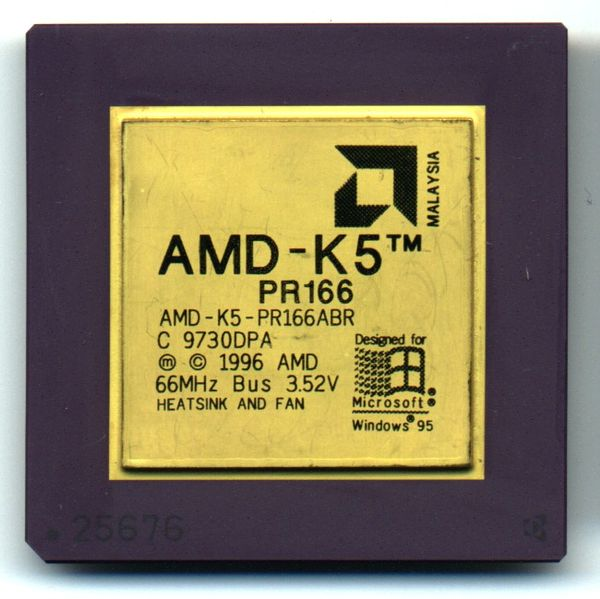
\includegraphics[scale = 0.8]{Graphics/amd-k5 PR166.jpg}
	\caption{\textbf{Microprocesador AMD K5 PR166}}
	\label{fig:27}
\end{figure}

\subsection{K6, Athlon, Duron y Sempron}
En 1995, \emph{AMD} adquirió \emph{NexGen} (fabricante de procesadores de arquitectura \textbf{RISC} principalmente) por los derechos de la serie \textbf{NX} de procesadores compatibles con x86. 
\emph{AMD} dio al equipo de diseño de \emph{NexGen} un edificio propio, los dejó solos, y les dio tiempo y dinero para reelaborar el \textbf{Nx686}. El resultado fue el procesador \textbf{K6}, 
introducido en 1995 y 1996. Aunque el \textbf{\textbf{K6}} se basó en el \textbf{Socket 7}, algunas versiones como el \textbf{K6-3/450} fueron más rápidas que el \textbf{Pentium II} de \emph{Intel}. 
El \textbf{K7} es el procesador de séptima generación x86 de \emph{AMD}, haciendo su debut el 23 de junio de 1999, bajo la marca \textbf{Athlon}. A diferencia de los procesadores anteriores de AMD, 
no podría ser utilizado en las mismas \emph{motherboards}, debido a problemas de licencia sobre el \textbf{Slot 1}(conector utilizado por algunos de los microprocesadores de \emph{Intel} como el \textbf{Pentium II})  
de \emph{Intel}, \emph{AMD} decide entonces usar como nombre la letra \textbf{A} que hace referencia al \emph{bus} del procesador \textbf{Alpha}. \emph{Duron} fue una versión limitada y de menor costo del \textbf{Athlon} (64KB en 
lugar de 256KB L2 de caché) con un \emph{socket} de \textbf{462-pin PGA (Socket A)} o soldado directamente a la \emph{motherboard}. \emph{Sempron} fue lanzado como un procesador \textbf{Athlon XP} de menor 
costo sustituyendo a \emph{Duron} en el \emph{socket} \textbf{A PGA}, desde entonces se fue manteniendo y actualizando esa línea hasta la llegada del  \emph{socket} \textbf{AM3}
\brackcite{sexton_2017_history_of_AMD_cpus,wikipedia_2022_amd}.

\subsection{K8}
\textbf{K8} es una gran revisión de la arquitectura \textbf{K7}, cuya mejora más notable es el agregado de extensiones de 64 bit sobre el conjunto de instrucciones x86. Esto es importante para \emph{AMD} puesto 
que marca un intento de definir el estándar x86 e imponerse, en vez de seguir los estándares marcados por \emph{Intel}. Y al respecto, \emph{AMD} ha tenido éxito. La historia dio un giro y 
Microsoft adoptó el conjunto de instrucciones de \emph{AMD}(AMD64), dejando a \emph{Intel} el trabajo de ingeniería inversa de las especificaciones de AMD (EM64T). Otras características notables de \textbf{K8} 
son el aumento de los registros de propósito general (de 8 a 16 registros), \textbf{Direct Connect Architecture} y el uso de \textbf{HyperTransport}
(tecnología de comunicaciones bidireccional, que funciona tanto en serie como en paralelo, y que ofrece un gran ancho de banda en conexiones punto a punto de baja latencia)
\brackcite{sexton_2017_history_of_AMD_cpus,wikipedia_2022_amd}.



\subsection{K10}
La próxima arquitectura de \emph{AMD}, \textbf{K10}, fue un diseño bastante ambicioso. Está estrechamente relacionado con el \textbf{K8}, pero tenía varias mejoras en el núcleo y en el controlador de memoria y caché asociado. 
El \textbf{IPC} se mejoró en comparación con \textbf{K8}, pero la mayor ventaja de \textbf{K10} fue su diseño de cuatro núcleos que le permitió sacar ventaja sobre las \textbf{CPU} de doble núcleo \textbf{K8} en aplicaciones con muchos subprocesos
\brackcite{sexton_2017_history_of_AMD_cpus,wikipedia_2022_amd}.

Desafortunadamente, el \textbf{K10} tuvo problemas desde el principio. Los primeros procesadores \textbf{K10} se basaron en la configuración de \emph{Barcelona} y se vendieron como procesador de servidor \textbf{Opteron}.

\subsection{Bulldozer}
En octubre de 2011, \emph{AMD} presentó el sucesor de su arquitectura \textbf{K10}, cuyo nombre en código es \emph{"Bulldozer"}. Con \emph{Bulldozer}, \emph{AMD} intentó utilizar una gran cantidad 
de núcleos y una velocidad de reloj superior para superar al recientemente lanzado \emph{Sandy Bridge}(Segunda generación de los \textbf{Intel Core}) de Intel. Sin embargo, el costo de este diseño 
centrado en la frecuencia del reloj fue una caída marcada en el \textbf{IPC} en comparación con la arquitectura \textbf{K10}. El primer chip \emph{Bulldozer}, con nombre en código \emph{Zambezi}, no pudo superar 
limpiamente a las \textbf{CPU} \textbf{Thuban Phenom II X6(K10)}, y mucho menos vencer a \emph{Sandy Bridge}.
El diseño fue criticado por consumir mucha energía y calentarse demasiado, aunque eso se deriva de comparaciones directas entre \emph{Bulldozer} y \emph{Sandy Bridge}
\brackcite{sexton_2017_history_of_AMD_cpus,wikipedia_2022_amd}.

\subsection{Ryzen: AMD renace}
\emph{AMD} perdió terreno frente a \emph{Intel} en prácticamente todas las áreas del mercado de \textbf{CPU} durante los años de \emph{Bulldozer}. 
La empresa perdió importantes recursos financieros y tuvo que vender sus fábricas de silicio. Con una batalla cuesta arriba para 
permanecer en el mercado de procesadores, \emph{AMD} puso sus esperanzas en \textbf{Ryzen}.
Bajo la microarquitecutra \emph{Zen}  en 2017 los primeros procesadores \textbf{Ryzen} salieron al mercado. 
\emph{Zen} es un diseño fresco que difiere de la antigua arquitectura \emph{Bulldozer}. Los microprocesadores basados en \emph{Zen} utilizan un proceso \textbf{FinFET} de 14 nm,  
son más eficientes energéticamente y pueden ejecutar muchas más instrucciones por ciclo. Se introduce \textbf{SMT}
(técnica para mejorar la eficiencia general de las \textbf{CPU} superescalares con subprocesos múltiples de hardware, similar al \textbf{Hyper-Threading} de \emph{Intel}), lo que permite que cada núcleo ejecute dos subprocesos
, aumentando el rendimiento del procesamiento mediante un mejor uso de los recursos disponibles.
El sistema de caché también ha sido rediseñado. En \textbf{Ryzen}, \emph{AMD} implementó por primera vez \emph{micro-op cache}, que permitía almacenar instrucciones usadas recientemente, 
lo que mejora el rendimiento y reduce las paradas del \emph{pipeline}.
Los procesadores \emph{Zen} también emplean sensores en todo el chip para escalar dinámicamente la frecuencia y el voltaje. Esto permite que el propio procesador defina de forma 
dinámica y automática la frecuencia máxima en función de la refrigeración disponible.
La microarquitectura \emph{Zen} logró una mejora del 52\% en \textbf{IPC} sobre \emph{Excavator}. 
El tope de gama de los \textbf{Ryzen} con microarquitecura \emph{Zen} : \textbf{Ryzen 7 1800X}, tenía ocho núcleos  a 3,6 GHz y podía acelerar hasta 4,1 GHz en ciertas cargas de trabajo 
\brackcite{sexton_2017_history_of_AMD_cpus,wikipedia_2022_amd,wikipedia_2022_zen}.

\begin{figure}[htb]
	\centering
	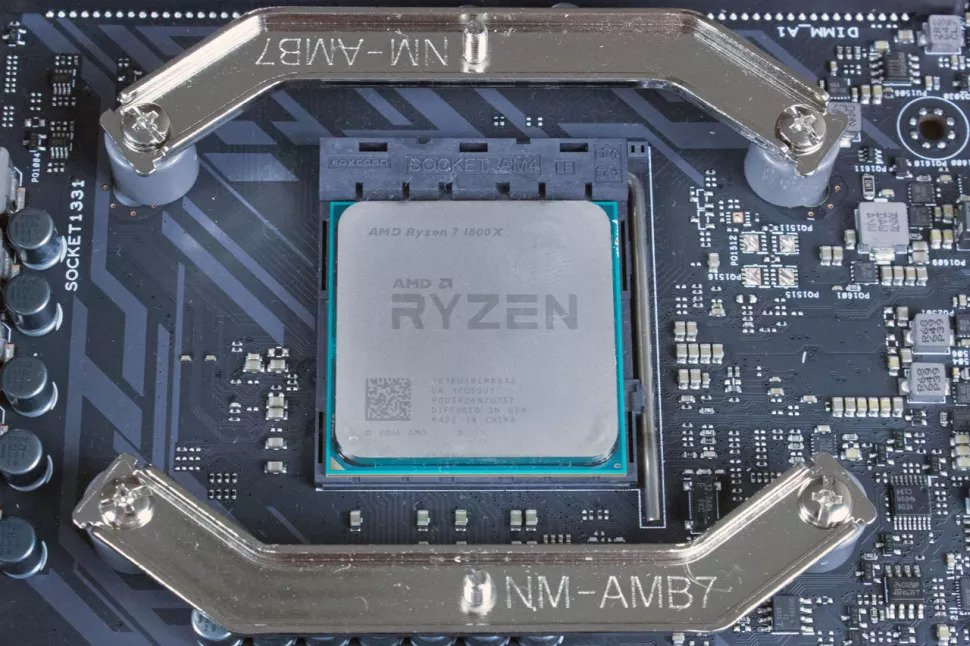
\includegraphics[scale = 0.4]{Graphics/ryzen 7 1800x.jpg}
	\caption{\textbf {Microprocesador} \textbf{Ryzen 7 1800x} puesto en el  \emph{socket} \textbf{AM4}}
	\label{fig:28}
\end{figure}

Las próximas generaciones  \emph{Zen 2} y \emph{Zen 3}  trajeron notables mejoras a los \textbf{Ryzen}. \emph{Zen 2} introdujo la arquitectura basada en \emph{chiplet}, 
en la que todas las microprocesadores de escritorio, estación de trabajo y servidor utilizaban los mismos \emph{chiplets} de núcleo. La principal ganancia 
de rendimiento de \emph{Zen 3} sobre \emph{Zen 2} es la introducción de un \textbf{CCX}(CPU-Complex) unificado, lo que significa que cada núcleo \textbf{chiplet} 
ahora se compone de ocho núcleos con acceso a 32 MB de caché, en lugar de dos conjuntos de cuatro núcleos con acceso a 16 MB de caché cada uno.
\brackcite{sexton_2017_history_of_AMD_cpus, wikipedia_2022_amd, wikipedia_2022_zen}.
